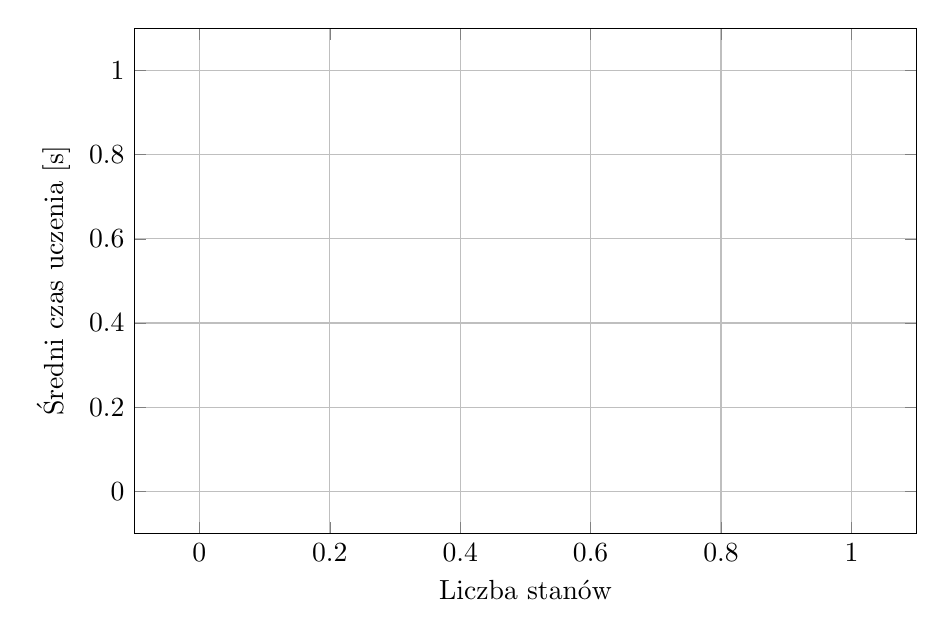
\begin{tikzpicture}
\begin{axis}[
    width=0.95\linewidth,
    height=8cm,
    xlabel={Liczba stanów},
    ylabel={Średni czas uczenia [s]},
    grid=major,
    legend style={at={(0.02,0.98)}, anchor=north west, font=\small},
    legend cell align=left
]
    \addplot[mark=*] coordinates { \DataTimeNoSrs };
    \addlegendentry{Średni całkowity czas uczenia bez SRS}

    \addplot[mark=square*] coordinates { \DataTimeSrs };
    \addlegendentry{Średni całkowity czas uczenia z SRS}
\end{axis}
\end{tikzpicture}